% Template for Cogsci submission with R Markdown

% Stuff changed from original Markdown PLOS Template
\documentclass[10pt, letterpaper]{article}

\usepackage{cogsci}
\usepackage{pslatex}
\usepackage{float}
\usepackage{caption}

% amsmath package, useful for mathematical formulas
\usepackage{amsmath}

% amssymb package, useful for mathematical symbols
\usepackage{amssymb}

% hyperref package, useful for hyperlinks
\usepackage{hyperref}

% graphicx package, useful for including eps and pdf graphics
% include graphics with the command \includegraphics
\usepackage{graphicx}

% Sweave(-like)
\usepackage{fancyvrb}
\DefineVerbatimEnvironment{Sinput}{Verbatim}{fontshape=sl}
\DefineVerbatimEnvironment{Soutput}{Verbatim}{}
\DefineVerbatimEnvironment{Scode}{Verbatim}{fontshape=sl}
\newenvironment{Schunk}{}{}
\DefineVerbatimEnvironment{Code}{Verbatim}{}
\DefineVerbatimEnvironment{CodeInput}{Verbatim}{fontshape=sl}
\DefineVerbatimEnvironment{CodeOutput}{Verbatim}{}
\newenvironment{CodeChunk}{}{}

% cite package, to clean up citations in the main text. Do not remove.
\usepackage{apacite}

% KM added 1/4/18 to allow control of blind submission


\usepackage{color}

% Use doublespacing - comment out for single spacing
%\usepackage{setspace}
%\doublespacing


% % Text layout
% \topmargin 0.0cm
% \oddsidemargin 0.5cm
% \evensidemargin 0.5cm
% \textwidth 16cm
% \textheight 21cm

\title{Interlocutors preserve complexity in language}


\author{Madeline Meyers \and Daniel Yurovsky \\
        \texttt{\{mcmeyers, yurovsky\}@uchicago.edu} \\
       Department of Psychology \\ University of Chicago}

\begin{document}

\maketitle

\begin{abstract}
Why do languages change? One possibility is they evolve in response to
two competing pressures: (1) to be easily learned, and (2) to be
effective for communication. In a number of domains (e.g.~kinship
categories, color terms), variation in the world's natural languages
appears to be accounted for by different but near-optimal tradeoffs
between these two pressures (Regier, Kemp, \& Kay, 2015). Models of
these evolutionary processes have modeled transmission chains in which
errors of learning by one agent become the language input for the
subsequent generation. However, a critical feature of human language is
that children do not learn in isolation. Rather, they learn in
communicative interactions with caregivers who can draw inferences from
their errorful productions to their intended interests. In a set of
iterated learning experiments, we show that this supportive context can
have a powerful stabilizing role in the development of artificial
languages, allowing them to achieve higher levels of asymptotic
complexity than they would by vertical transmission alone.

\textbf{Keywords:}
communication; language acquisition; language evolution; iterated
learning
\end{abstract}

\hypertarget{introduction}{%
\section{Introduction}\label{introduction}}

How do you ask a group of people where they are going in Spanish? In
Spain, the answer depends on the group: you might ask ``Donde van
ustedes?'' of a group of work colleagues, but to address your friends,
you use the informal ``Donde váis vosotros?'' instead. In Mexican
Spanish, this distinction has disappeared, and the ``ustedes'' form is
used exclusively. Why did Spanish change in this way, simplifying and
shedding the formal second person plural? One working theory is that
languages evolve to adapt to two dynamic competing pressures: (1) ease
of learning and transmission, and (2) effective communication (Lupyan \&
Dale, 2010).

When children are learning language, they often make simplification
errors (Bowerman, 1982). If a child is asking for her bottle, she may be
unable to produce the canonical English label ``bottle,'' and say
``baba'' instead. Because her caregivers can combine her errorful
utterance with their beliefs about what she wants, they can nonetheless
correctly interpret this as a request for the bottle.

\textbf{STILL THINKING THROUGHT THIS, I DON'T THINK THIS IS QUITE RIGHT}

This simplification works well, until the child starts to learn her
animal words, and calls a sheep ``baba''. Here, she is conforming to the
language-learnability bias: if she calls both a bottle and a sheep
``baba'', she has one less word to remember. Does this child go through
life believing that ``baba'' is the label for these disparate objects?
It's possible. Perhaps, if she never has a need to discriminate between
sheep and bottles, she might even pass this label on to her children. In
this way, errors in language can be passed on to the next generation
through transmission from one speaker to the next. This process reflects
the needs of the language speakers: if a distinction between objects is
not needed for effective communication, there is no need to retain
complexity.

Children are often the actors who drive language evolution (Senghas,
2003), yet they differ from adults in their cognitive capabilities,
namely, memory systems (Kempe, Gauvrit, \& Forsyth, 2015), interests and
early vocabularies, and conversation partners. Even though children are
skilled language learners, their developing cognitive systems prevent
aspects of language that are difficult to learn and remember from being
passed on -- pushing languages towards simplicity (Hudson Kam \&
Newport, 2005; Senghas, 2003). But languages that become too simple can
lose the ability to be effective for communication (Kirby, Griffiths, \&
Smith, 2014). Indeed, we could not have ``baba'' become the label for
every object. What enables languages to retain their communicative
utility in the face of these learnability pressures?

Most Americans grow up in a world where it is useful to discriminate
sheep and bottles -- and they must learn the different labels for these
objects. It is often caregivers, through their explicit interventions as
well as their implicit modeling of correct language, who may be
reintroducing descriptiveness into a language where it would otherwise
be lost. Children's language learning is greatly influenced by those
around them -- especially the adults they talk to most. These caregivers
control much of their child's linguistic input, and are responsible for
seeing that their children develop effective and useful systems of
communication. Even the youngest children are not passive learners of
language --- they are active participants, engaging in conversations
with their parents. These adults are experts both in the language and in
the children themselves, as they understand the child's intuitions,
personality, and context. Caregivers play an important interpretive role
in these interactions through their ability to understand the intended
target of children's errorful productions (Chouinard \& Clark, 2003).
Adults can explicitly correct their children's language errors in
various ways (e.g., by interruptions or repeating the correct
word/grammatical form) (Penner, 1987). Yet, children primarily learn
language through listening to others talk, rather than explicit
instruction (Romberg \& Saffran, 2010). Thus, parent's modeling of
accurate language constructions can have a powerful effect on reducing
children's language errors: over time, children fix their own mistakes
because they have learned the correct constructions from their
caregivers (Hudson Kam \& Newport, 2005). By way of this feedback, both
implicit and explicit, children's simplification errors are corrected,
and children are able to acquire adult-like speech. Eventually, when a
child grows to be an adult, they will not transmit the errors they had
as a child, but the correct forms of speech they learned from their
caregivers -- as long as learning the correct forms is useful and
necessary. Thus, over the course of a lifetime, the child language
learner grows to become a parent language teacher, correcting their own
children's errors. These error reconstructions may be a mechanism by
which more structure is retained in language over many lifetimes than
children could sustain alone.

\hypertarget{using-iterated-learning-to-study-language-change}{%
\subsection{Using iterated learning to study language
change}\label{using-iterated-learning-to-study-language-change}}

To model the impact of these competing pressures on language evolution
in the laboratory, we use the iterated learning paradigm developed by
Kirby et al. (2014). In this paradigm, one participant is trained on a
randomly-generated language--e.g, a set of words created by arbitrarily
pairing syllables together. That participant is later asked to recall
the language, but inevitably makes some errors. This participants'
errorful output then becomes the input for the next participant,
producing a transmission chain. This iterated learning process models
the transmission of language across generations, with each participant
unintentionally changing the language through their memory biases.

This paradigm has been used productively across a number of studies of
this kind of cross-generational transmission in both adults (e.g., Smith
\& Wonnacott, 2010; Christiansen \& Kirby, 2003; Kirby, Dowman, \&
Griffiths, 2007; Kirby et al., 2014; structure \& signals, 2014), and
children (Kempe et al., 2015; Raviv \& Arnon, 2018). A few more recent
studies have also compared languages evolved over multiple generations
(vertical transmission) to languages evolved by iterated use in the same
conversational partners (horizontal transmission, Kirby, Tamariz,
Cornish, \& Smith, 2015). However, participants in horizontal
transmission had similar levels of knowledge and similar cognitive
constraints. Children learning language in asymmetric knowledge
situations, where their parent both knows more language and has an adult
cognitive system (Figure \ref{fig:baseline_schem}). We predict that this
asymmetry may have a unique role in the evolution of language, allowing
languages to resist some of the simplifying pressure of ease of
transmissibilty through adults' ability to keep structure in place
temporarily while children develop.

We adapted Kempe et al. (2015)'s non-linguistic iterated learning
paradigm to model the effect of introducing a secondary,
error-correcting participant on the evolution of language. We
hypothesize that these error-correctors (analogous to caregivers and
teachers) are pivotal not only to an individual's successful language
acquisition, but also to the evolution of the language as a whole. This
is because those who correct mistakes and provide feedback are able to
protect against the strong transmissibility (simplicity) bias in early
language learners by re-introducing and preserving complexity in
language.

All experiments were pre-registered on Open Science Framework, and all
data and code can be accessed at the following link:
\url{https://osf.io/guzyf/?view_only=43ee3fe87cf24c968c4377675c3bc580}.

\begin{CodeChunk}
\begin{figure}[tb]

{\centering 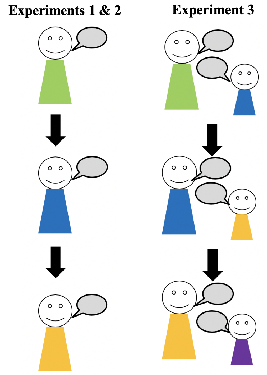
\includegraphics{figs/baseline_schem-1} 

}

\caption[In Experiments 1 and 2 follow the conventional iterated learning paradigm, where a novel language is transmitted vertically through successive learning and recall]{In Experiments 1 and 2 follow the conventional iterated learning paradigm, where a novel language is transmitted vertically through successive learning and recall. In Experiment 3, an element of horizontal transmission is added to the paradigm: novel language learners' reproductions are subject to feedback from a secondary participant, and this production is passed to the subsequent learner.}\label{fig:baseline_schem}
\end{figure}
\end{CodeChunk}

\hypertarget{experiment-1-replicating-kempe-2015}{%
\section{Experiment 1: Replicating Kempe et al.
(2015)}\label{experiment-1-replicating-kempe-2015}}

We began by replication Kempe, Gauvrit, and Forsyth's (2015) experiment
using a nonlinguistic stimulus to study the evolution of structure. We
had two motivations for using this paradigm. First, the structures in
this paradigm lend themselves to algorithmic quantification of
complexity. Second, Kempe et al. (2015) used this paradigm successfully
with children, and our goal was to test our hypothesis not just in
adult-adult chains, but also in child-adult chains (ongoing).

\hypertarget{method}{%
\subsection{Method}\label{method}}

\hypertarget{participants}{%
\subsubsection{Participants}\label{participants}}

Participants in Experiment 1 were 120 adults recruited on Amazon
Mechanical Turk. These participants were dived into twenty diffusion
chains, each of which had six generations. Each participant gave
informed consent. The task was approximately eight minutes long, and
subjects were compensated \$0.50 for their participation.

\hypertarget{design-and-procedure}{%
\subsubsection{Design and Procedure}\label{design-and-procedure}}

Participants in Experiment 1 were asked to re-create patterns on a grid.
Subjects were informed that they would see a target grid appear on their
computer screen for ten seconds, followed by a picture (a visual mask)
displayed for three seconds. After the visual mask, participants viewed
a blank 8x8 grid where they were given one minute to re-create the
target grid. Participants could click on any cell in the grid to change
its color, and could also remove any color placed. A counter on the
screen showed how many cells had been colored, and it varied dynamically
with the participant's clicks. After placing 10 colors, participants
could click a button to advance to the next trial (See Figure
\ref{fig:e2_withplots} for example grids). A timer was also displayed on
the screen, and participants were given an audio cue when they had
fifteen seconds left.

Prior to completing one training and three practice trials, each
participant completed 6 Experiment trials. Participants in the first
generation of each chain received the same initial grids for Experiment
trials. These initial 8x8 grids were generated by randomly selecting 10
of the 64 possible cells to be filled. Participants in subsequent
generations received as their targets the outputs produced by the
previous participant in their chain. All participants received the same
training and practice trials. In the preliminary training trial,
subjects viewed two 8x8 grids side-by-side and were instructed to make
the blank grid on the right match the target grid on the left.
Participants were unable to progress to the practice and Experimental
trials without reaching perfect accuracy on this first trial.

Participants' performance on the practice trials were used as an
attention check to determine whether their data would be passed to the
next participant. If the participant scored less than 75\% accuracy on
the last two practice trials, or if they failed to select 10 cells
before time ran out, their outputs were not transmitted to the next
generation. In Experiment 1, five participants failed to meet these
criteria and were excluded from analysis.

\hypertarget{analysis}{%
\subsection{Analysis}\label{analysis}}

Our primary measures of interest were reproduction accuracy and pattern
complexity. Reproduction accuracy serves as a proxy for transmissibility
-- higher reproduction accuracies indicate that the ``language'' is
easier to learn. Reproduction accuracy was computed as the proportion of
targets out of 10 which were placed in the same location on the target
and input grids.

Complexity served as a proxy for descriptiveness. We followed Kempe et
al. (2015) in using several measures of complexity: algorithmic
complexity, chunking, and edge length. Algorithmic complexity is
calculated using the Block Decomposition Method, a measure of
Kolmogorov-Chaitin Complexity applied to 2-dimensional patterns (Zenil,
Soler-Toscano, Dingle, \& Louis, 2014). This measure computes the length
of the shortest Turing machine program required to produce the observed
pattern. The shorter the program, the simpler the pattern. Chunking is
the number of groups of colored blocks which share an edge. The more
groups of blocks, the easier the pattern is to transmit, and the lower
its complexity is. Edge length is the total perimeter of the colored
blocks. If all blocks were in one chunk, the edge length would be low,
and the complexity of the pattern would be lower compared to if none of
the chosen targets shared an edge. Implementation of these metrics was
adapted from code provided by Gauvrit, Soler-Toscano, \& Guida (2017).

\hypertarget{results-and-discussion}{%
\subsection{Results and Discussion}\label{results-and-discussion}}

If iterated learning captures the hypothesized pressures of
expressiveness and transmissibility, we predict that reproduction
accuracy should increase, and complexity should decrease over
generations. We tested these predictions with mixed-effects logistic
regressions, predicting accuracy and all three measures of complexity
separately from fixed effects of generation and trial number, and random
intercepts for participant and initial grid (e.g.
\texttt{accuracy $\sim$ generation + trial +  (1|subject) + (1|initialGrid)}.

Reproduction accuracy increased significantly over generations
(\(\beta =\) 0.033, \(t =\) 3.146, \(p =\) .002). Figure
\ref{fig:e1_acc_plot} shows the results for accuracy. Complexity on all
three measure decreased significantly over generations, as shown by
Figure \ref{fig:e1_bdm_plot} (\(\beta_{BDM} =\) -3.219, \(t =\) -6.696,
\(p =\) \textless{} .001; \(\beta_{chunking} =\) -0.35, \(t =\) -6.499,
\(p =\) \textless{} .001; \(\beta_{edge} =\) -0.763, \(t =\) -6.662,
\(p =\) \textless{} .001). Trial Number, or how far along the subject
was in the task, was not a significant predictor in any model.

In line with Kempe et al. (2015), we found that accuracy increased cross
generations and complexity decreased on all three measures. However,
this changed appeared to be non-linear, with later generations perhaps
evolving less rapidly than later generations (Figure
\ref{fig:e1_acc_plot}). We thus replicated this experiment again, but
increased the number of generations from six to twelve to have the power
to estimate the shape of the evolutionary functions.

\begin{CodeChunk}
\begin{figure}[tb]

{\centering 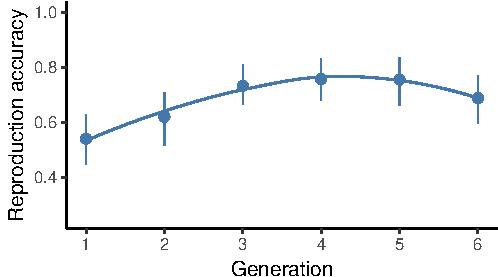
\includegraphics{figs/e1_acc_plot-1} 

}

\caption[Experiments 1 show increases in accuracy (measured by proportion of 10 targets placed correctly) across transmission generations]{Experiments 1 show increases in accuracy (measured by proportion of 10 targets placed correctly) across transmission generations.}\label{fig:e1_acc_plot}
\end{figure}
\end{CodeChunk}

\begin{CodeChunk}
\begin{figure}[tb]

{\centering 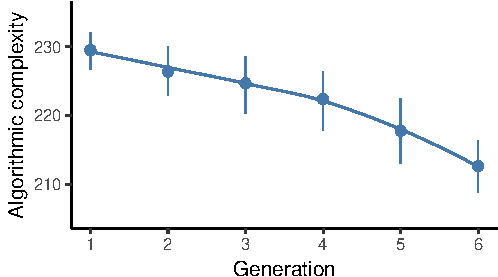
\includegraphics{figs/e1_bdm_plot-1} 

}

\caption[Experiment 1 shows decreases in algorithmic complexity (measured by the Block Decomposition Method) across transmission generations]{Experiment 1 shows decreases in algorithmic complexity (measured by the Block Decomposition Method) across transmission generations.}\label{fig:e1_bdm_plot}
\end{figure}
\end{CodeChunk}

\hypertarget{experiment-2-replication-and-extension-of-experiment-1}{%
\section{Experiment 2: Replication and extension of Experiment
1}\label{experiment-2-replication-and-extension-of-experiment-1}}

Experiment 2 replicated the task from Experiment 1 with the addition of
twice as many chains and generations. The purpose of this replication
was primarily to approximate the shape of the algorithmic complexity
curve.

\hypertarget{method-1}{%
\subsection{Method}\label{method-1}}

\hypertarget{participants-1}{%
\subsection{Participants}\label{participants-1}}

Participants in Experiment 2 were 519 adults recruited on Amazon
Mechanical Turk. These participants were dived into forty diffusion
chains, each of which had twelve generations. Each participant gave
informed consent and was compensated with \$0.50 for their participation
in this 8-minute task.

\hypertarget{design-and-procedure-1}{%
\subsection{Design and Procedure}\label{design-and-procedure-1}}

The task in Experiment 2 was identical to Experiment 1. Participants
were told to reproduce patterns on a grid, and their responses were
passed to the next subject in the transmission chain.

Approximately 8\% (n=39) of participants in Experiment 2 were excluded
from analysis due to failure to meet accuracy requirements on the
practice trials or failure to select the complete number of cells on one
or more experimental trials. This resulted in a total of 480
participants included in the analysis.

\hypertarget{results}{%
\subsection{Results}\label{results}}

The results of this experiment replicated those found in Experiment 1.
Reproduction accuracy increased significantly over generations, as shown
by Figure \ref{fig:e2_acc_plot} (\(\beta =\) 0.01, \(t =\) 6.029,
\(p =\) \textless{} .001).

Figure \ref{fig:e2_withplots} shows the results for algorithmic
complexity. Algorithmic complexity appeared to follow an exponential
function of the form \(y = e^{-x} + b\). We therefore fit an exponential
mixed-effects regression model predicting complexity from fixed effects
of generation and trial number, and random intercepts for participant,
and initial grid (e.g.
\texttt{log(complexity) $\sim$ log(generation+1) + trial + (1|subject) + (1|initial)}).
Algorithmic complexity decreased and asymptoted over generations
(\(\beta_{BDM} =\) -7.307, \(t =\) -10.998, \(p =\) \textless{} .001).
Similar trends were also found with chunking and edge length, the
alternate measures of complexity (\(\beta_{chunking} =\) -0.693, \(t =\)
-14.955, \(p =\) \textless{} .001; \(\beta_{edge} =\) -1.375, \(t =\)
-13.11, \(p =\) \textless{} .001). As in Experiment 1, Trial Number was
not a significant predictor in any model.

\begin{CodeChunk}
\begin{figure}[tb]

{\centering 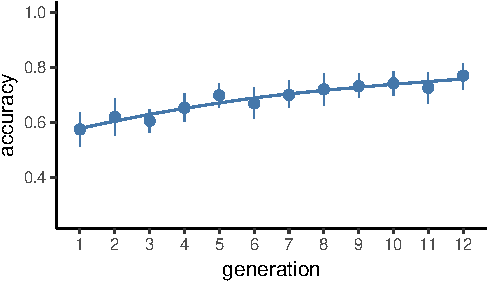
\includegraphics{figs/e2_acc_plot-1} 

}

\caption[Experiment 2 shows increases in transmission accuracy over generations]{Experiment 2 shows increases in transmission accuracy over generations.}\label{fig:e2_acc_plot}
\end{figure}
\end{CodeChunk}

\begin{CodeChunk}
\begin{figure}[tb]

{\centering 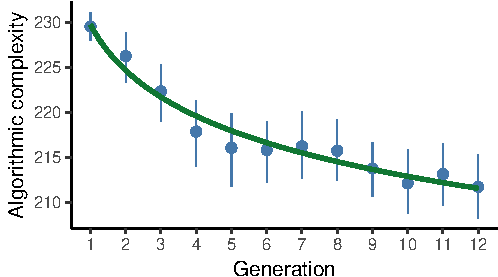
\includegraphics{figs/e2_bdm_plot-1} 

}

\caption[Experiments 1 and 2 show increases in accuracy over transmission generations.CHANGE POINT SIZE]{Experiments 1 and 2 show increases in accuracy over transmission generations.CHANGE POINT SIZE}\label{fig:e2_bdm_plot}
\end{figure}
\end{CodeChunk}

\hypertarget{experiment-3-introducing-an-interlocutor}{%
\section{Experiment 3: Introducing an
interlocutor}\label{experiment-3-introducing-an-interlocutor}}

In order to add an element of feedback from a more experienced
interlocutor to the iterated-learning process, we adapted the task from
Experiments 1 and 2 to include a secondary, ``editing'' participant.
This participant was analogous to a caregiver who protects their child
from acquiring and perpetuating incorrect linguistic forms.

\hypertarget{method-2}{%
\subsection{Method}\label{method-2}}

\hypertarget{participants-2}{%
\subsection{Participants}\label{participants-2}}

Participants in Experiment 3 were 1031 adults recruited on Amazon
Mechanical Turk. These participants were dived into forty diffusion
chains, each of which had twelve generations. Each participant gave
informed consent and was compensated with \$0.50 for their
participation.

\hypertarget{design-and-procedure-2}{%
\subsection{Design and Procedure}\label{design-and-procedure-2}}

In the third, dyad experiment, a primary participant was designated to
be a ``learner'' and completed the same task as in Experiment 1 and
Experiment 2. They were told to re-produce patterns on a grid. A
secondary participant -- the ``fixer'' -- was given an adapted task.
Throughout the study, fixers were not told to re-create patterns, but to
fix patterns to resemble a target grid exactly. Fixers in this
experiment viewed the same target grid as learners, but instead of
seeing an empty input grid, they saw a grid with 10 elements filled in
-- the elements that the previous learner had submitted. The participant
could then edit the 10 items' positions. There was no ``reset'' button
during this task, so data reflect participants' initial instincts.

In Experiment 3, a generation consisted of a learner, who re-created the
target grid, and a fixer, who then received the same target grid as well
as the learner's input grid to edit. The fixer's edited pattern was used
as the target grid for the subsequent generation.

Approximately 8\% (n=71 of participants in Experiment 3 were excluded
from analysis due to failure to meet accuracy requirements on the
practice trials or failure to select the necessary number of targets on
one or more experimental trials. This resulted in a total of 960
participants included in the analysis.

\hypertarget{analysis-and-results}{%
\subsection{Analysis and Results}\label{analysis-and-results}}

As in Experiments 1 and 2, our primary measures of analysis were
accuracy and complexity. These measures were computed using the same
methods as in the previous experiments.

Fixers and learners had significantly different pattern reproduction
accuracies \ref{fig:dyad_accuracy}. According to a linear mixed-effects
model predicting group from generation and Trial Number and controlling
for random effects of subject and initial grid. Reproduction accuracies
between groups were significantly different
(\(\beta_{condition-child} =\) -0.086, \(t =\) -11.338, \(p =\)
\textless{} .001). Neither the fixers' or learners' transmission
accuracies increased significantly over generations
(\(\beta_{fixers} =\) 0.007, \(t =\) 1.108, \(p =\) .269;
\(\beta_{learners} =\) 0.011, \(t =\) 1.706, \(p =\) .089).

\ref{fig:e3_complexity_condition} shows the relationship between the
complexity of fixers' and learners' patterns. In each generation, the
learner decreases the complexity of the pattern, and the fixer is able
to compensate for some of this loss. AS in Experiment 2, we fit an
exponential model to the data. Both conditions show decreases in pattern
complexity over generations (\(\beta_{learners} =\) -0.021, \(t =\)
-4.572, \(p =\) \textless{} .001; \(\beta_{fixers} =\) -0.014, \(t =\)
-6.183, \(p =\) \textless{} .001), although the effect of generation is
stronger for learners compared to fixers (\(\beta_{generation} =\)
-3.648, \(t =\) -10.117, \(p =\) \textless{} .001). These results hold
true for all three measures of complexity \emph{DO ALL OF THESE STATS
NEED TO BE PUT IN}.

\ref{fig:both_complexity} shows that the presence of an editor does help
retain complexity in the grid patterns. The addition of a fixer into the
task allowed a higher degree of complexity to be retained in the
language over time (\(\beta_{condition-child} =\) -3.66, \(t =\) -6.296,
\(p =\) \textless{} .001). Additionally, the patterns in the dyad
condition asymptoted earlier than in the baseline condition \emph{(Stats
for this?)}.

\begin{CodeChunk}
\begin{figure}[tb]

{\centering 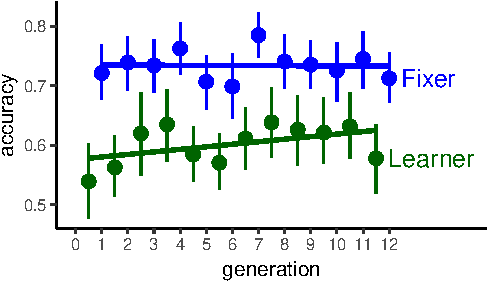
\includegraphics{figs/dyad_accuracy-1} 

}

\caption[In Experiment 3, fixers show significantly higher reproduction accuracies than learners]{In Experiment 3, fixers show significantly higher reproduction accuracies than learners. Reproduction accuracies stay relatively constant, although the accuracies of the learners increase across generations.}\label{fig:dyad_accuracy}
\end{figure}
\end{CodeChunk}

\begin{CodeChunk}
\begin{figure}[tb]

{\centering 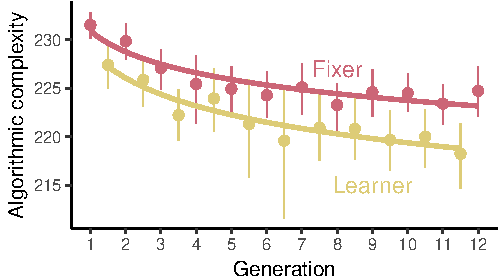
\includegraphics{figs/e3_complexity_condition-1} 

}

\caption[In Experiment 3, algorithmic complexity decreases and asymptotes for both Learners and Fixers]{In Experiment 3, algorithmic complexity decreases and asymptotes for both Learners and Fixers. Learners have consistently lower complexity values compared to Fixers.}\label{fig:e3_complexity_condition}
\end{figure}
\end{CodeChunk}

\begin{CodeChunk}
\begin{figure}[tb]

{\centering 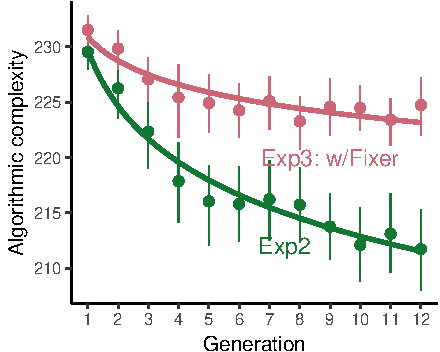
\includegraphics{figs/both_complexity-1} 

}

\caption[The fixer's reproductions from Experiment 3 show greater levels of algorithmic complexity across generations compared to the participants' reproductions from Experiment 2]{The fixer's reproductions from Experiment 3 show greater levels of algorithmic complexity across generations compared to the participants' reproductions from Experiment 2.}\label{fig:both_complexity}
\end{figure}
\end{CodeChunk}

\hypertarget{general-discussion}{%
\section{General Discussion}\label{general-discussion}}

Despite the use of a non-linguistic task in Experiments 1-3, we were
able to measure change in a culturally-transmitted, learned symbol
system. In Experiments 1 and 2, language simplified rapidly and
dramatically, reflecting the strong pressure towards simplification in
language learning. These findings replicated those of Kempe et al.
(2015): when transmitting an artificial language of grid patterns,
complexity in the language was lost.

However, the results of Experiment 3 show that this loss is not cultural
regression, as complexity can be reintroduced in the language by way of
a secondary participant. When the iterated-learning process begins to
resemble the true process of language-learning, where children speak
with and are subject to correction by those more competent in the
language, a lesser amount of complexity was lost during transmission.
Additionally, this stable level of complexity was much higher, and was
reached earlier in the transmission chain with the help of a fixing
participant. This stability in complexity did not mean that the language
stopped changing, but that the descriptiveness and transmissibility
pressures were in balance. Fixers in Experiment 3 represented caregivers
-- they were more accurate at reproducing the language, and could
therefore be seen as more fluent speakers, just as adults are of their
native languages. The learners, on the other hand, had a more difficult
task, which greater strained their working memories, similar to the
strain on a child language learner who is inundated with new words each
day. The fixer's corrected language was passed to the next learner in
the chain, representing a child who, after many years of being corrected
by their own parent, becomes a parent, and, in turn, passes their
optimal language to the next generation. Due to the higher accuracy by
fixers, and therefore greater knowledge of the language, the fixers were
able to compensate for some (not all) of the learners' losses in
complexity.

When a caregiver or teacher prevents their child from growing up to
believe that ``baba'' is the word for both ``bottle'' and ``sheep'',
they are not only helping their individual child become a competent
speaker of the language, but they are also reintroducing complexity,
thus helping the language system as a whole from simplifying to disuse.
Data collection is ongoing with children ages 6-8 at a local science
museum in both the Experiment 1 and Experiment 3 tasks, in order to
investigate whether the pressures of similarity and complexity affect
children similarly to how they affect adults in early language-learning
conditions.

We do not learn language as passive listeners, who absorb a proportion
of the linguistic input they hear. Therefore, we cannot measure language
learning only through measuring input, nor through measuring only
linguistic output. Languages are both learned and changed through
conversations to evolve to the needs of the language's users. Therefore,
we must study language learning in process, to see how it adapts and
evolves with communicative interactions.

\hypertarget{references}{%
\section{References}\label{references}}

\setlength{\parindent}{-0.1in} 
\setlength{\leftskip}{0.125in}

\noindent

\hypertarget{refs}{}
\leavevmode\hypertarget{ref-bowerman-1982}{}%
Bowerman, M. (1982). U shaped behavioral growth. In (pp. 101--145).
Academic Press.

\leavevmode\hypertarget{ref-chouinard-2003}{}%
Chouinard, M. M., \& Clark, E. V. (2003). Adult reformulations of child
errors as negative evidence. \emph{Journal of Child Language},
\emph{30}(3), 637--669.

\leavevmode\hypertarget{ref-christiansen-2003}{}%
Christiansen, M. H., \& Kirby, S. (2003). Language evolution. In M. H.
Christiansen \& S. Kirby (Eds.), (pp. 1--15). Oxford University Press.

\leavevmode\hypertarget{ref-gauvrit-2017}{}%
Gauvrit, N., Soler-Toscano, F., \& Guida, A. (2017). A preference for
some types of complexity comment on ``perceived beauty of random texture
patterns: A preference for complexity''. \emph{Acta Psychologica},
\emph{174}, 48--53.

\leavevmode\hypertarget{ref-hudsonkam-2005}{}%
Hudson Kam, C. L., \& Newport, E. L. (2005). Regularizing unpredictable
variation: The roles of adult and child learners in languagae formation
and change. \emph{Language Learning and Development}, \emph{1}(2),
151--195.

\leavevmode\hypertarget{ref-kempe-2015}{}%
Kempe, V., Gauvrit, N., \& Forsyth, D. (2015). Structure emerges faster
during cultural transmission in children than in adults.
\emph{Cognition}, \emph{136}, 247--254.

\leavevmode\hypertarget{ref-kirby-2007}{}%
Kirby, S., Dowman, M., \& Griffiths, T. L. (2007). Innateness and
culture in the evolution of language. \emph{Proceedings of the National
Academy of Sciences}, \emph{104}(12), 5241--5245.

\leavevmode\hypertarget{ref-kirby-2014}{}%
Kirby, S., Griffiths, T., \& Smith, K. (2014). Iterated learning and the
evolution of language. \emph{Current Opinion in Neurobiology},
\emph{28}, 108--114.

\leavevmode\hypertarget{ref-kirby-2015}{}%
Kirby, S., Tamariz, M., Cornish, H., \& Smith, K. (2015). Compression
and communication in the cultural evolution of linguistic structure.
\emph{Cognition}, \emph{141}, 87--102.

\leavevmode\hypertarget{ref-lupyan-2010}{}%
Lupyan, G., \& Dale, R. (2010). Language structure is partly determined
by social structure. \emph{PLoS ONE}, \emph{5}(1), 1--10.

\leavevmode\hypertarget{ref-penner-1987}{}%
Penner, S. G. (1987). Parental responses to grammatical and
ungrammatical child utterances. \emph{Child Development}, \emph{58}(2),
376--384.

\leavevmode\hypertarget{ref-raviv-2018}{}%
Raviv, L., \& Arnon, I. (2018). Systematicity, but not compositionality:
Examining the emergence of linguistic structure in children and adults
using iterated learning. \emph{Cognition}, \emph{181}, 160--173.

\leavevmode\hypertarget{ref-regier2015}{}%
Regier, T., Kemp, C., \& Kay, P. (2015). 11 word meanings across
languages support efficient communication. \emph{The Handbook of
Language Emergence}, \emph{87}, 237.

\leavevmode\hypertarget{ref-romberg-2010}{}%
Romberg, A. R., \& Saffran, J. (2010). Statistical learning and language
acquisition. \emph{WIREs Cognitive Science}, \emph{1}, 906--914.

\leavevmode\hypertarget{ref-senghas-2003}{}%
Senghas, A. (2003). Intergenerational influence and ontogenetic
development in the emergence of spatial grammar in nicaraguan sign
language. \emph{Cognitive Development}, \emph{18}, 511--531.

\leavevmode\hypertarget{ref-smith-2010}{}%
Smith, K., \& Wonnacott, E. (2010). Eliminating unpredictable variation
through iterated learning. \emph{Cognition}, \emph{116}, 444--449.

\leavevmode\hypertarget{ref-verhoef-2014}{}%
structure, E. of combinatorial, \& signals. (2014). Verhoef, tessa and
kirby, simon and de boer, bart. \emph{Journal of Phonetics}, \emph{43},
57--68.

\leavevmode\hypertarget{ref-zenil-2014}{}%
Zenil, H., Soler-Toscano, F., Dingle, K., \& Louis, A. A. (2014).
Correlation of automorphism group size and topolical properties with
program-size complexity evaluations of graphs and complex networks.
\emph{Physica A}, \emph{404}, 341--358.

\bibliographystyle{apacite}


\end{document}
